\documentclass[10pt]{article}
\usepackage{geometry}
\geometry{a4paper, margin=1in}
\usepackage{setspace}
\setstretch{1.25}
\usepackage{titlesec}
\newcommand{\indexsection}[1]{\section{#1}\index{#1}}
\newcommand{\indexsubsection}[1]{\subsection{#1}\index{#1@\thesection~#1}}
\usepackage{pgfgantt}
\usepackage{float}
\usepackage{graphicx}
\usepackage[portuguese]{babel}
\usepackage{url}
\usepackage{indentfirst}
\usepackage{subcaption}

\usepackage{imakeidx}
\graphicspath{ {./images/} }

\makeindex[columns=1, title=Contents, intoc]
\begin{document}

\begin{titlepage}
    \begin{center}
        \vspace*{1cm}

    {\fontsize{17}{16}\selectfont \textbf{Design and development of a dispatch board for public transport operators based on web technologies (PE43)}}

        \vspace{0.5cm}
        Capstone Project Final Report

        \vspace{1.5cm}

        \textbf{António Ferreira} \\
        \textbf{Cristiano Rocha} \\
        \textbf{José Ferreira} \\
        \textbf{Pedro Magalhães} \\

                \vfill

        
\includegraphics[width=0.4\textwidth]{UPORTO_fundotransparente}


        Bachelor of Informatics and Computer Engineering

        \vspace{0.8cm}

        \textbf{U.Porto Tutor:} Teresa Galvão \\
        \textbf{Proponent:} Thiago Sobral \\

    \vspace{0.4cm}
        Date: 2024-06-21

    \end{center}
\end{titlepage}

\thispagestyle{empty}
\clearpage

\thispagestyle{empty}
\tableofcontents

\clearpage

\section{Introduction}
    This report aims to provide an overview of our project that involved the implementation of a system for a dispatch board for public transport operators.

    \subsection{Background}
    The project was carried out within the OPT facilities (Otimização e Planeamento de Transportes S.A). We were accompanied by our tutor from OPT, Thiago Sobral, who guided us through the entire work and helped us with everything we needed.

    \subsection{Objectives and Expected Results}
        The main motivation behind this project was the need to upgrade the already existing software used to display the dispatch board to a programming language that could be more easily managed, maintaining the existing features, and database integration.
        
        The existing software was considered outdated and hard to deploy since it ran natively on the devices, every update and bugfix required a manual software update of all the machines that needed it.

        The development of this dispatch board was based on an existing program, our job was to upgrade it by:
        \begin{itemize}
            \item adapting it to a web-based language, so that it is easier to expand and debug, taking advantage of the best and most recent tools of web-dev;
            \item adding customizations and “quality of life” features to improve the overall usability of the product.
        \end{itemize}

        Here is an example of the old dispatch board, it was a native application that ran on the machines of the transport operators, it was hard to maintain and expand, and it was not user-friendly. It was also not responsive and that is why the printscreen looks like it is cut off.
        
        \vfill
        \begin{figure}[!ht]
            \centering
            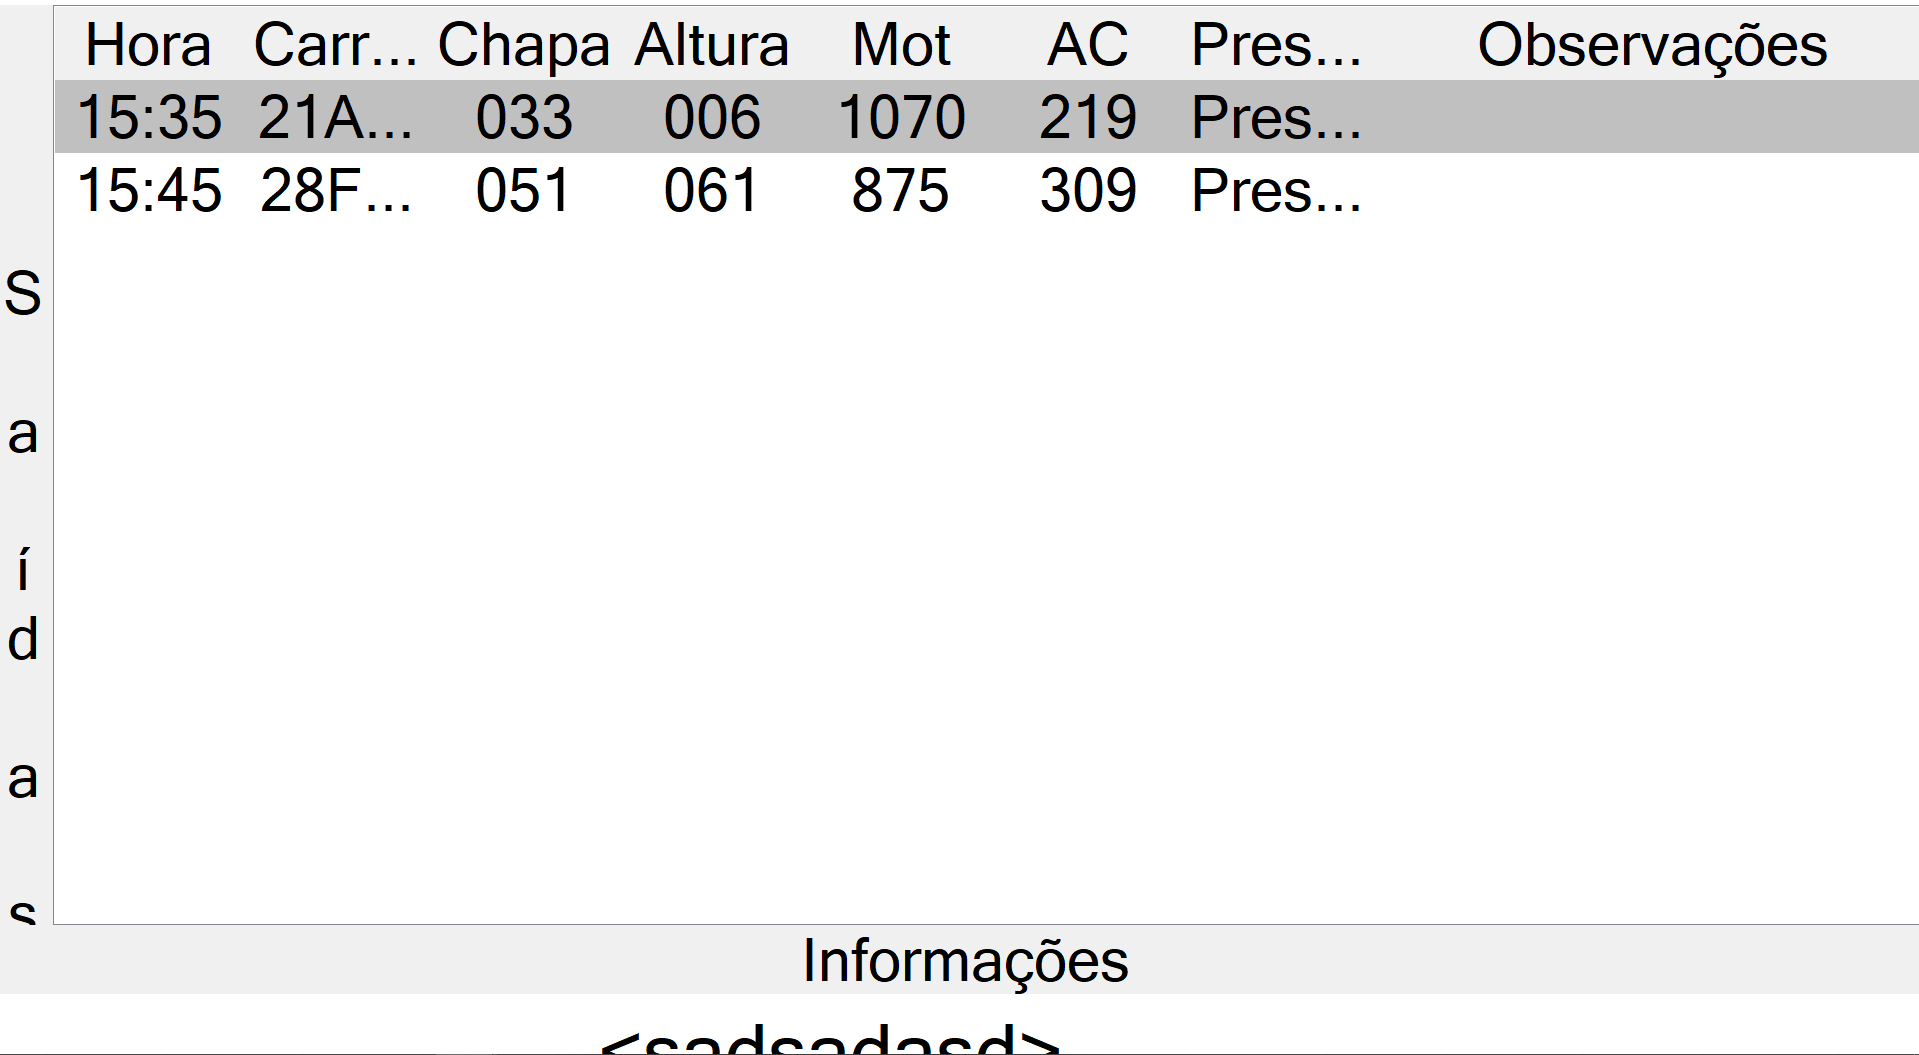
\includegraphics[width=1\textwidth]{old_dispatch_board}
            \caption{Old dispatch board}
            \label{fig:old_dispatch_board}
        \end{figure}
        
    \subsection{Report Structure}
        This report will have the following structure:
        \begin{itemize}
            \item     \textbf{Introduction:} Brief description of the initial background, motivation and context behind the project and the expected results.
            \item     \textbf{Methodology and Development Process:} Description of the methodologies and main activities that were carried out in this project, including the methodology that was used, the intervenients and their roles/responsibilities, and the main activities that were developed during the project.
            \item     \textbf{Solution Development:} The requirements and restrictions of the final product and the architecture and technologies used.
            \item     \textbf{Conclusion:} Conclusion of the report with a summary of what we as a group achieved with this project and what we learned.
        \end{itemize}

\section{Methodology and Development Process}

    \subsection{Methodology}
        
        To ensure consistent progress and receive regular feedback, our group established a weekly meeting schedule with our OPT tutor. These meetings allowed us to review our work, discuss any challenges, and make necessary adjustments based on the feedback received.
        
        For version control and collaboration, we utilized GitHub. We created a repository where we committed our code, which greatly enhanced our communication and organization. This platform allowed us to track changes, manage different versions of our project, and work simultaneously without conflicts.
        
        Our online meetings were conducted through a Discord group we created specifically for this project. We utilized both text and voice chat features to communicate in real-time while working on the project. Additionally, we included our OPT tutor in the Discord group so he could monitor our progress and provide feedback directly within this collaborative environment.
        
        For coding, we chose Visual Studio Code as our primary editor. This tool offered an array of extensions and features that facilitated our development process, making it easier to write, debug, and collaborate on our code efficiently.

    \subsection{Stakeholders and roles}
        Several people were involved in the project, each with specific roles and responsibilities. The stakeholders and their roles are as follows:
        \begin{itemize}
            \item Project Team(4 members):
            \begin{itemize}
                \item António Ferreira: Frontend Developer
                \item Cristiano Rocha: Frontend Developer
                \item José Ferreira: Frontend Developer
                \item Pedro Magalhães: Backend Developer
            \end{itemize}
            \item Project Coordinators:
            \begin{itemize}
                \item Professor and advisor Thiago Sobral from OPT: Responsible for advising and mentoring us, providing expertise and guidance.
                \item Professor and supervisor Maria Teresa Galvão Dias from FEUP: Oversees the project and provides guidance and feedback.
                \item Professor and Director of Capstone Project (Projeto Integrador) Nuno Flores: Conductor of Projeto Integrador.
            \end{itemize}
            \item Project Users:
            \begin{itemize}
                \item Transport Operators: The primary users of the dispatch board system.
            \end{itemize}
        \end{itemize}

    \subsection{Activities Developed}
        During the project’s duration, several activities took place, such as planning, coding and team meetings.

        \begin{itemize}
            \item \textbf{Planning:}
            \begin{itemize}
                \item     The initial phase involved determining the technologies to be used. In a meeting with our OPT coordinator, we decided on Node.js and Prisma for the backend, and React with TypeScript for the frontend.
                \item     We also discussed the project's requirements and constraints, such as the need for real-time updates and the importance of maintaining the existing features.
                \item     After the initial planning, we began the requirement analysis, which involved understanding the existing system and identifying the features that needed to be implemented in the new dispatch board. We consulted with our OPT coordinator to ensure that the new system met the required specifications.
            \end{itemize}
            \item \textbf{Development:}
            \begin{itemize}
                \item     The development phase began with setting up the project structure and creating the initial files. We were provided a database from one of the existing dispatch board systems, which we used to test the backend. We were also provided the queries used to retrieve the data from the database.
                \item     We then proceeded to implement the backend, focusing on the database connection and API endpoints. We used Prisma to interact with the database and Next.js to create the API routes.
                \item     Another important aspect was the implementation of a way to customize the dispatch board, allowing users to change the colors and layout and the logo according to their preferences. We decided to use a JSON file to store these customizations, so that the users could export and import their settings to other devices.
                \item     The frontend development followed, with the creation of the user interface and integration with the backend. We used React with TypeScript to build the frontend, focusing on the real-time updates and customization features. There was a focus on creating a simple and intuitive interface that would be easy to use by the transport operators.
            \end{itemize}
            \item \textbf{Testing:}
            \begin{itemize}
                \item We conducted several rounds of testing to ensure that the system was functioning correctly and that all features were working as expected. We tested the real-time updates and customization options to verify that they were working properly.
                \item We also conducted user testing with the transport operators to gather feedback on the system's usability and identify any issues that needed to be addressed.
            \end{itemize}
        \end{itemize}

        Here's a Gantt chart showing the project's timeline, as it can be seen, the project was divided into 3 main phases: Planning, Implementation, Testing and Documentation, but we added a few more tasks to better represent the activities that were developed.

        After the initial planning, we began the requirement analysis, which involved understanding the existing system and identifying the features that needed to be implemented in the new dispatch board. We consulted with our OPT coordinator to ensure that the new system met the required specifications.

        The development phase began with setting up the project structure and creating the initial files. We were provided a database from one of the existing dispatch board systems, which we used to test the backend. We were also provided the queries used to retrieve the data from the database.

        We then proceeded to implement the backend, focusing on the database connection and API endpoints. We used Prisma to interact with the database and Next.js to create the API routes.

        Another important aspect was the implementation of a way to customize the dispatch board, allowing users to change the colors and layout and the logo according to their preferences. We decided to store the user settings on the local storage, so that the users could export and import their settings to other devices.

        \begin{figure}[h!]
            \centering
            \begin{ganttchart}[
                hgrid,
                vgrid,
                x unit=0.5cm,
                title/.style={fill=gray!30, draw=none},
                title label font=\footnotesize,
                bar/.style={fill=blue!30, draw=none},
                bar height=0.7,
                bar label font=\footnotesize,
                group/.style={fill=green!30, draw=none},
                group right shift=0,
                group top shift=0.7,
                group height=.3,
                group peaks width={0.2},
                milestone/.style={fill=red!50, draw=none},
                milestone height=0.7
            ]{1}{16}
                \gantttitle{2024}{16} \\
                \gantttitle{March}{4}
                \gantttitle{April}{4}
                \gantttitle{May}{4}
                \gantttitle{June}{4} \\
                \ganttgroup{Planning}{1}{4} \\
                \ganttbar{Requirement Analysis}{1}{2} \\
                \ganttlinkedbar{System Design}{3}{4} \ganttnewline
                \ganttmilestone{Design Review}{4} \ganttnewline
                \ganttbar{Implementation}{5}{11} \\
                \ganttlinkedbar{Testing}{12}{14} \\
                \ganttlinkedmilestone{Deployment}{14} \ganttnewline
                \ganttbar{Documentation}{12}{14}
            \end{ganttchart}
            \caption{Chart}
            \label{fig:chart}
        \end{figure}
        

\section{Solution Development}

    \subsection{Requirements}
        The main requirements for the dispatch board system were as follows:
        \begin{itemize}
            \item Functional Requirements:
                \begin{itemize}
                    \item \textbf{Customization:} The system should allow users to customize the dispatch board according to their preferences, such as changing the colors, logo and layout(display the columns that they consider useful and hide the ones that are considered useless for that company, also switch the order of the columns).
                    \item \textbf{User-friendly interface:} The system should have a simple and intuitive interface that is easy to use by the transport operators.
                    \item \textbf{Database integration:} The system should be able to connect to a database to retrieve the necessary information about the buses and schedules.
                    \item \textbf{Modular architecture:} The system should be modular, allowing for easy expansion and maintenance. It should also be possible for many transportation companies to use the same system, with each one having its own customizations and schedules.
                \end{itemize}
            \item Non-functional Requirements:
                \begin{itemize}
                    \item \textbf{Reliability:} The system should be reliable, with real-time updates ensuring that the transport operators have access to the most up-to-date information.
                    \item \textbf{Usability:} The system should be easy to use, with a user-friendly interface that is intuitive and accessible to all transport operators. This is especially important for operators who may not be familiar with technology. The system should also be in Portuguese, as most of the transport operators don't speak English.
                    \item \textbf{Performance:} The system should be fast and responsive, with minimal lag or delay when loading the schedules. This is crucial for transport operators who need to access the information quickly and efficiently.
                    \item \textbf{Scalability:} The system should be scalable, able to handle a large number of users and schedules without compromising performance. This is important as the system may be used by multiple transportation companies simultaneously.
                    \item \textbf{Lightweight:} The system should be lightweight, with minimal resource requirements. This is important as the system may be used on older devices with limited processing power or lightweight raspberry pi-like devices.
                \end{itemize}
            \item Constraints:
                \begin{itemize}
                    \item \textbf{Web-app based:} The system should tings from a JSON file.be developed as a web application, so that it can be accessed from any device with a web browser.
                    \item \textbf{Keep the existing features:} The system should maintain the existing features of the dispatch board, such as displaying the buses'/trains' schedules.
                    \item \textbf{Real-time updates:} The system should provide real-time updates, ensuring that the transport operators have access to the most up-to-date information.
                \end{itemize}
            \item Assumptions:
                \begin{itemize}
                    \item The transport operators have access to a device with a web browser, such as a computer or tablet.
                    \item The transport operators have a basic understanding of technology and can navigate a web application.
                \end{itemize}
            \item Dependencies:
            \begin{itemize}
                \item The system depends on the database to retrieve the necessary information about the schedules.
            \end{itemize}
        \end{itemize}
        \subsection{Architecture and Technologies}

        \subsubsection{Technology choice and reasoning}
        Before embarking on the development of the dispatch board system, careful consideration was given to defining the optimal architecture and technologies. 
        
        The selection of these components was crucial to ensure scalability, reliability, and ease of maintenance, while aligning with the project requirements and existing systems.
        
        With the freedom to choose the technologies, extensive research and discussions were conducted to make informed decisions. After thorough evaluation, the following technologies were deemed most suitable for the project:
        \begin{itemize}
                \item \textbf{Web Framework:}
                \begin{itemize}
                    \item \textbf{Description:} Next.js is a popular web framework for building modern and responsive user interfaces. It is built on top of React, a JavaScript library for building user interfaces, and provides additional features and optimizations specifically designed for server-side rendering and static site generation.
                    \item \textbf{Reasoning:} Next.js was chosen for its flexibility in rendering strategies, performance optimizations, and ease of development. It offers a modern and fast user interface, making it a perfect fit for this project.
                \end{itemize}

                \item \textbf{Frontend:}
                \begin{itemize}
                    \item \textbf{Technology:} React with TypeScript was chosen for the frontend development. TypeScript is a superset of JavaScript that adds static typing to the language, providing enhanced code quality and improved developer productivity. React is a powerful library for building user interfaces, offering a component-based architecture that simplifies the development process.
                    \item \textbf{Reasoning:} React's component-based architecture simplifies the development process and enhances code quality. TypeScript adds static typing to JavaScript, providing improved code quality and developer productivity.
                \end{itemize}

                \item \textbf{Backend:}
                \begin{itemize}
                    \item \textbf{Description:} We utilized an existing SQL Server database for the project, which contained the necessary information about the buses and schedules.
                    \item \textbf{Reasoning:} The SQL Server database provided by OPT was a suitable choice for the project as it already contained the necessary information about the buses and schedules. Leveraging this existing database allowed us to focus on developing the frontend and backend components without the need to create a new database from scratch.
                \end{itemize}

                \item \textbf{ORM (Object-Relational Mapping):}
                \begin{itemize}
                    \item \textbf{Description:} Prisma is an advanced ORM that simplifies database interactions by providing a type-safe and intuitive API. It supports multiple databases, including PostgreSQL, SQL Server, MySQL, and SQLite, making it a versatile and efficient choice for the project.
                    \item \textbf{Reasoning:} Prisma was selected for simplified database interactions and data manipulation. It is easy to utilize in Next.js and offers a seamless solution for the project's data handling needs.
                \end{itemize}
        \end{itemize}


        \subsubsection{Architecture}
        The architecture of the dispatch board system was designed to be easy to maintain, easy to use, and efficient. 
        
        It consists of three main components: the frontend, backend, and database. 
        
        These components work together to provide a seamless user experience for transport operators, ensuring real-time updates and customization options. 
        
        To represent the architecture, we created a layer diagram that illustrates the interaction between the components.

        \begin{figure}[h]
            \centering
            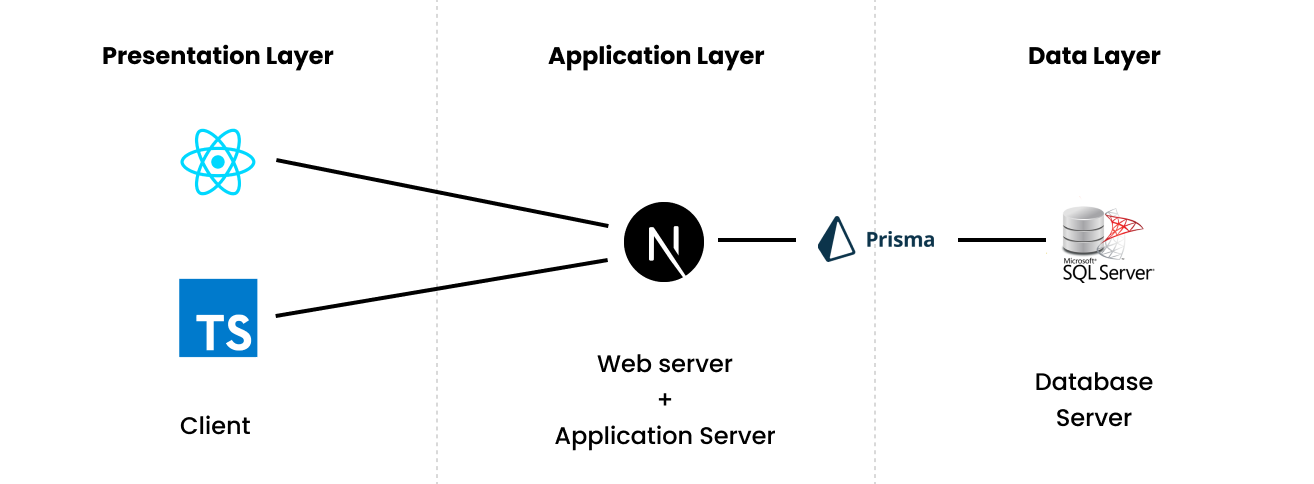
\includegraphics[width=1\textwidth]{architecture_diagram}
            \caption{Layer diagram of the dispatch board system architecture}
            \label{fig:architecture_diagram}
        \end{figure}

        \subsubsection{Difficulties encountered and their resolution}
        At the start of the project, we encountered difficulties with the initial setup. We initially considered creating a Docker container to deploy the project and the database in a local environment, ensuring consistency across team members. However, after conducting research and some trial and error, we determined that this would introduce unnecessary complexity.

        Fortunately, OPT provided us with a pre-existing database, eliminating the need to create one from scratch and simulate data. However, we faced the challenge of communicating with the database from both inside and outside of OPT. There were two different methods of connecting to the database, requiring manual changes to the .env file.

        To address this issue, we developed a console executable file that automates the switching between environments, simplifying the process for seamless communication.
        \subsection{Developed Solution}

        \subsubsection{Wireframes}
        Before starting the development of the dispatch board system, we created wireframes to visualize the layout and design of the application. These wireframes served as a blueprint for the final product, ensuring consistency and alignment with the project requirements.

        We presented the wireframes to our OPT coordinator for feedback and approval, ensuring that the design met the necessary specifications. The wireframes provided a clear visual representation of the application's structure and functionality, guiding the development process and ensuring a cohesive user experience.

        \begin{figure}[htbp]
            \centering
            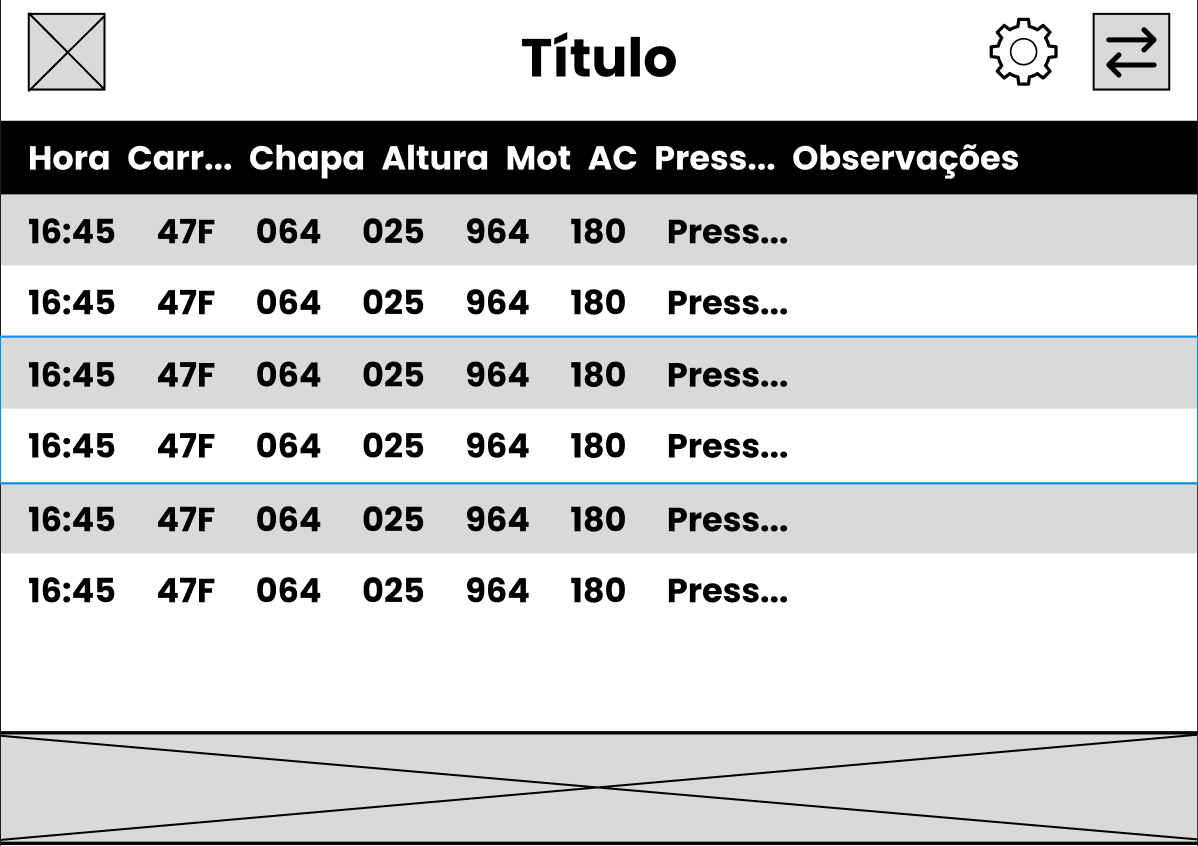
\includegraphics[width=1\textwidth]{wireframe}
            \caption{Wireframes of the dispatch board system}
            \label{fig:wireframes}
        \end{figure}
        

        \subsubsection{Home page}

        Our home page offers a streamlined navigation experience, presenting three key options: Table of Entries, Table of Exits, and Settings Page. Each option is represented by a dedicated button for quick access. Simply click on a button to be redirected to the corresponding page, allowing for efficient management and customization of transport operations. This intuitive interface ensures users can easily navigate to the desired section with minimal effort.

        \vfill
        \begin{figure}[htbp]
            \centering
            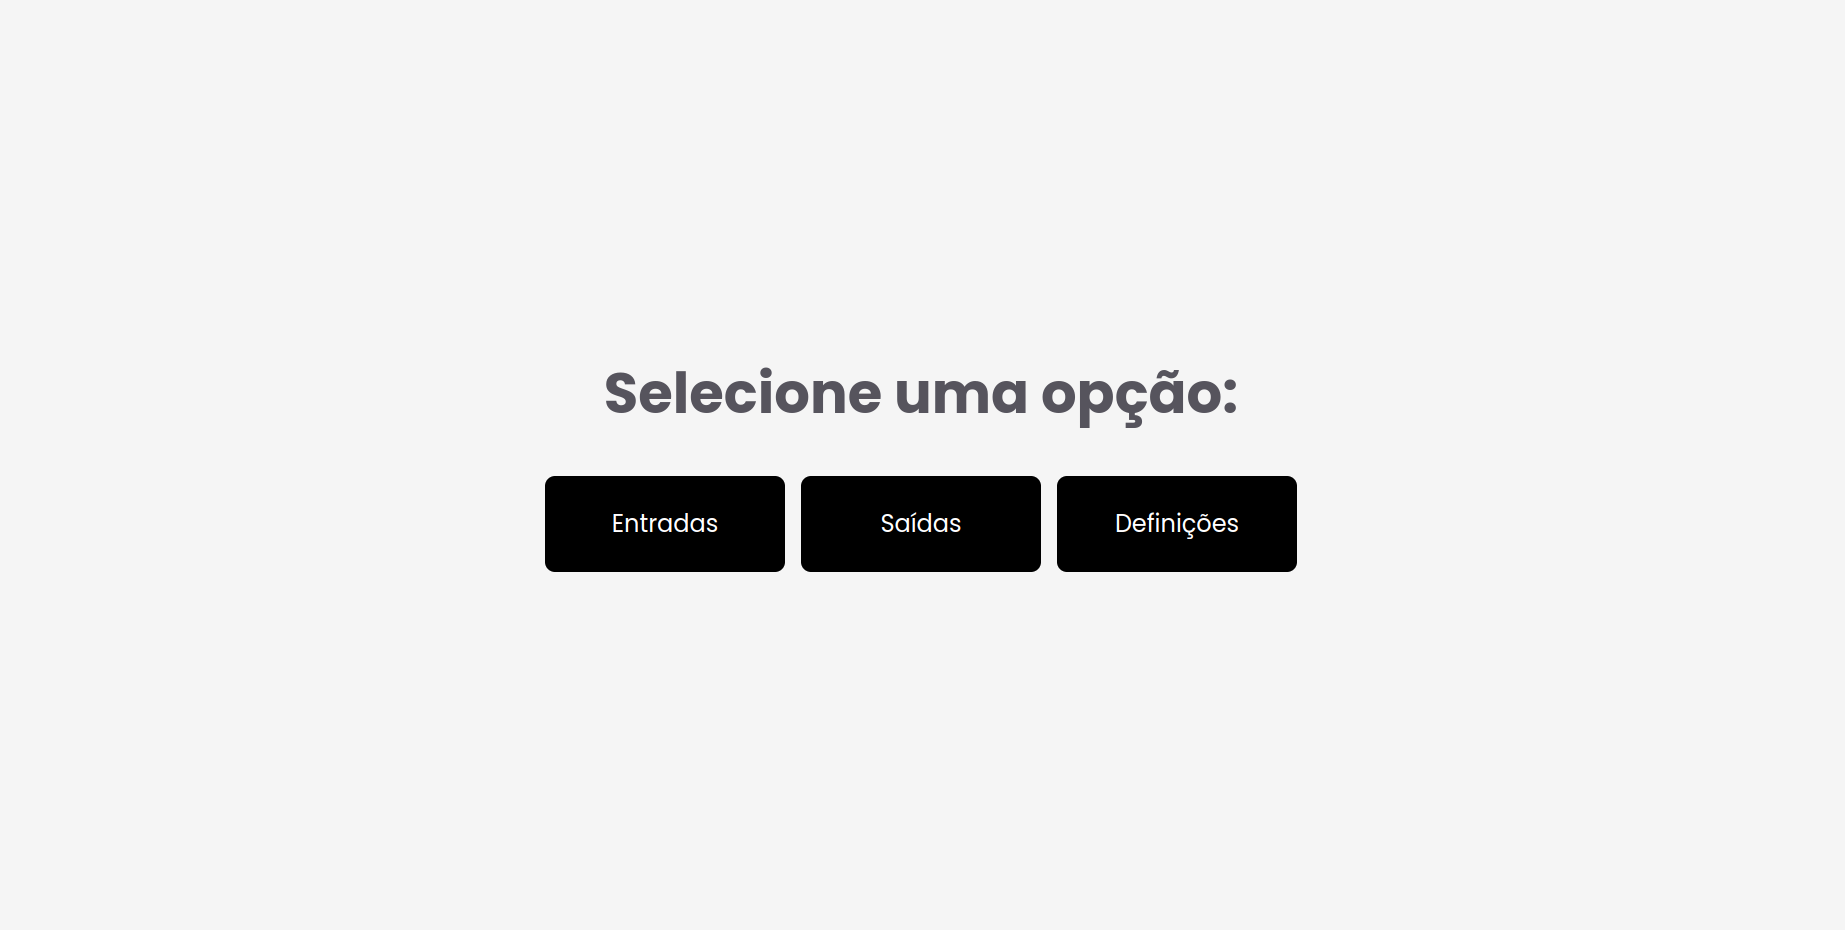
\includegraphics[width=1\textwidth]{home_page}
            \caption{Home page of the dispatch board system}
            \label{fig:home_page}
        \end{figure}

        \subsubsection{Table of entries and exits}

        We developed a comprehensive table of entries, encompassing all the necessary information for transport operators. 
        
        Leveraging the existing table model used by OPT, we undertook a meticulous redesign to enhance its modernity, appeal, and user-friendliness. This revamped table features a header displaying the logo of the company utilizing the application, along with intuitive options for toggling between the table of entries and the table of exits.
        
        Additionally, users can easily navigate to the settings page, where they have access to a variety of customization options. These settings allow users to tailor the application's appearance and functionalities according to their preferences, including the ability to enable or disable specific features.
        
        The table dynamically displays all transport schedules from the current time until the end of the day, with real-time updates ensuring accuracy and reliability. Users are provided with clear visual cues, such as a red highlight for any delayed transport schedules, facilitating efficient and effective transport management. This system not only enhances operational efficiency but also significantly improves the user experience for all stakeholders involved.
       
        At the bottom of the page, there is an area dedicated to displaying the most recently updated information by the application user. This feature enables users to promptly report incidents such as road accidents, ensuring timely dissemination of critical information.

        \begin{figure}[htbp]
            \centering
            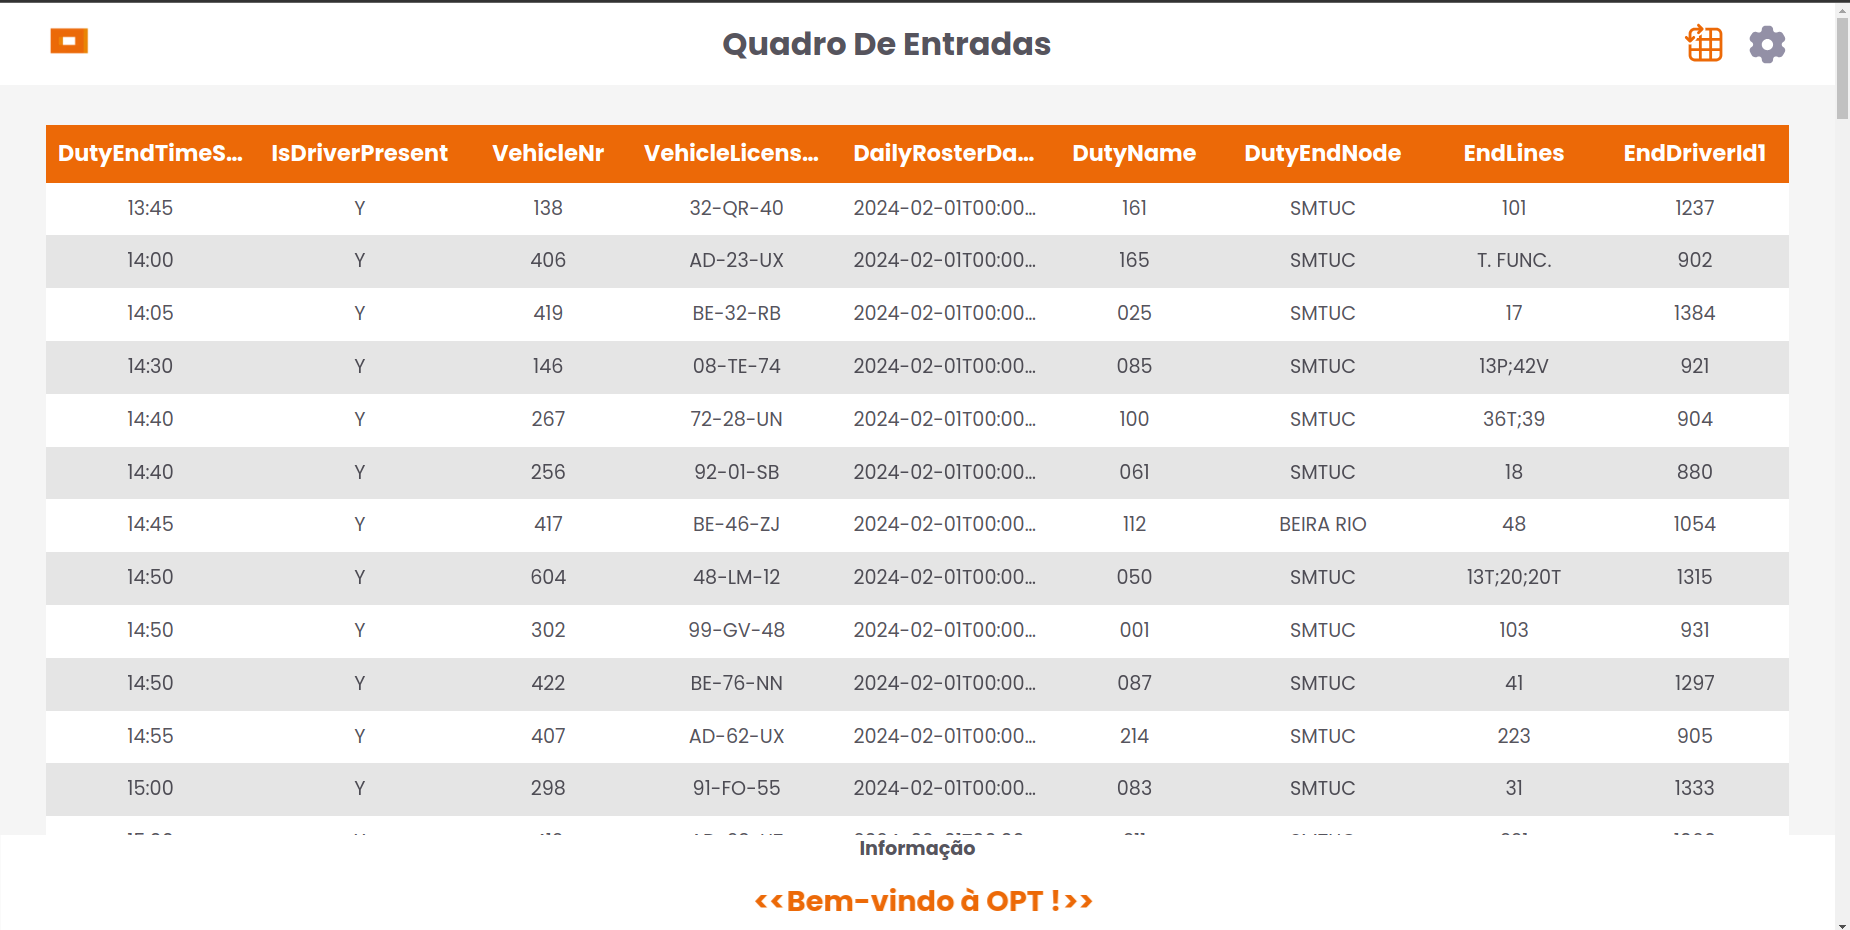
\includegraphics[width=1\textwidth]{table_of_entries}
            \caption{Table of entries in the dispatch board system}
            \label{fig:table_of_entries}
        \end{figure}
        \vfill

        \begin{figure}[htbp]
            \centering
            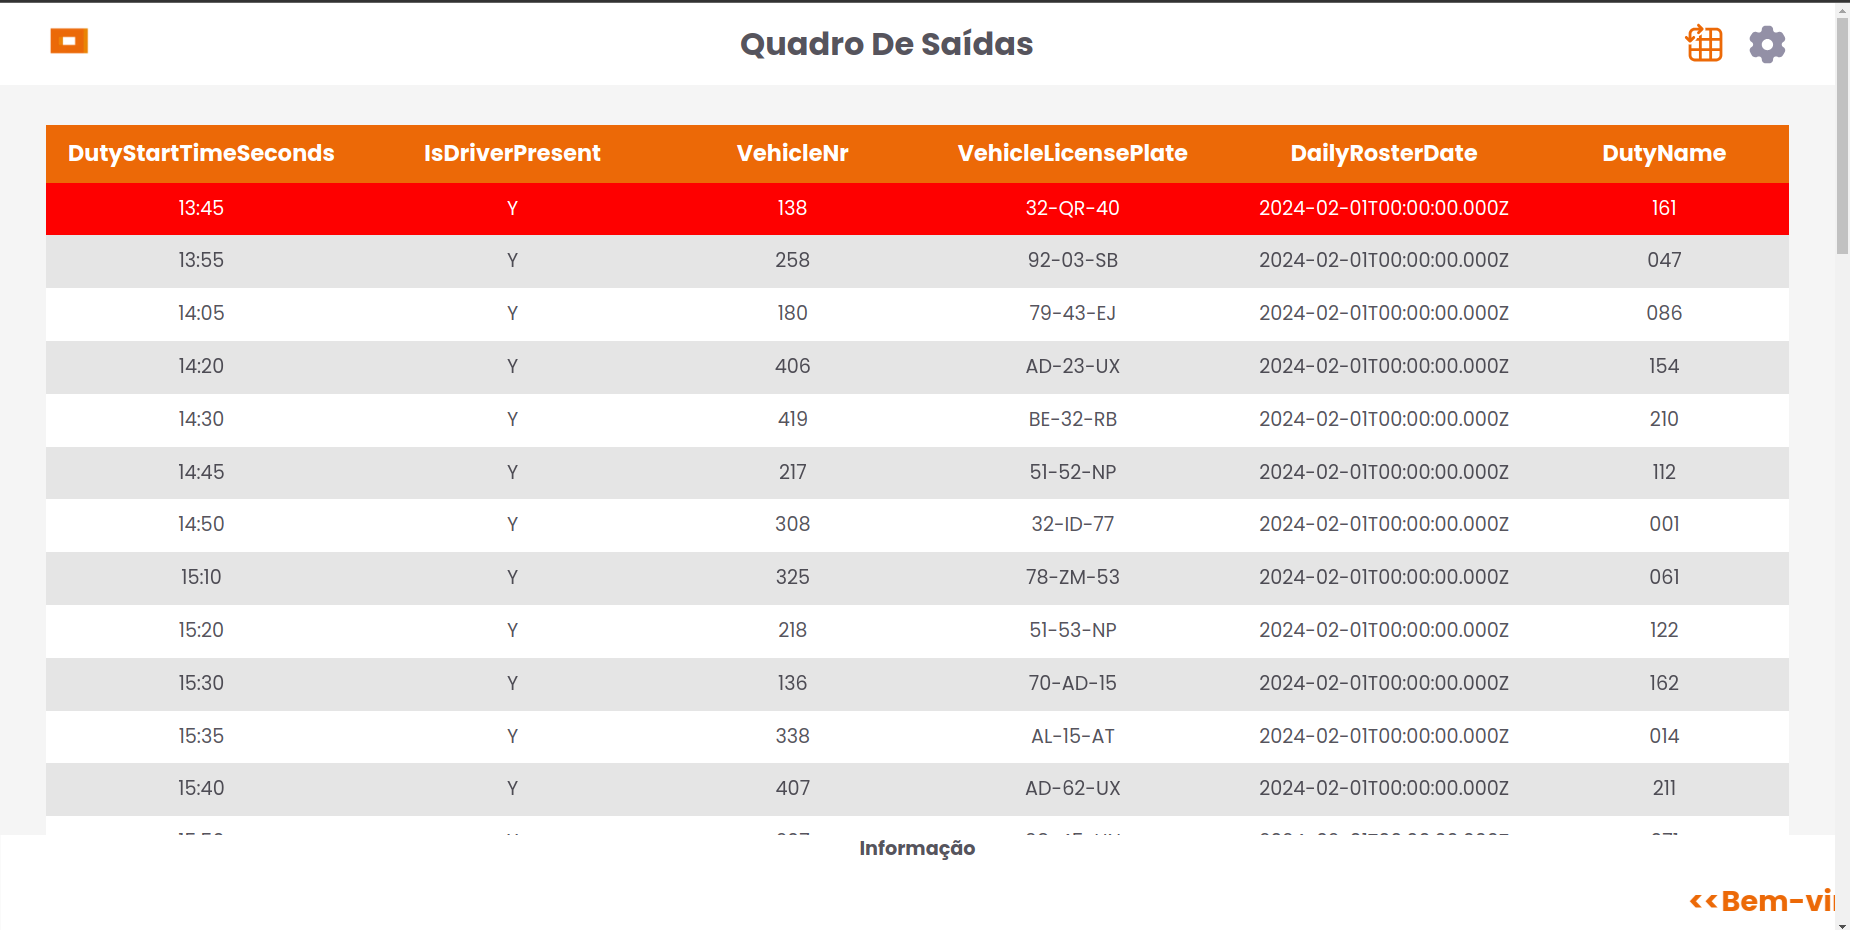
\includegraphics[width=1\textwidth]{table_of_exits}
            \caption{Table of exits in the dispatch board system}
            \label{fig:table_of_exits}
        \end{figure}

        \subsubsection{Settings page}

        Our settings page offers extensive customization options tailored to enhance user interaction. A sleek color selection bar allows precise configuration of highlighting, primary and secondary backgrounds, as well as primary and secondary text colors. 
        
        Each option triggers a color picker for seamless color selection and adjustment.
        Users can upload a company logo effortlessly using a dedicated upload button. For configuration management, the page includes export/import functionality for saving and reapplying settings as a JSON file. 
        
        A preview section provides a live demonstration of layout changes, ensuring users can visualize and confirm adjustments to entry and exit tables before finalizing.
        This comprehensive approach ensures a personalized and intuitive experience, empowering users to tailor the application's appearance and functionality to their exact specifications.
        
        The second settings page focuses on fine-tuning table display and content preferences. Users have granular control over column visibility, allowing them to show or hide specific columns as needed. Additionally, columns can be renamed to align with specific data or organizational needs.
        Display order customization empowers users to arrange columns in a preferred sequence, optimizing data presentation. 
        
        Furthermore, users can modify the information displayed at the bottom of entry and exit tables, ensuring relevance and clarity.
        This page serves as a powerful tool for configuring and optimizing data presentation, enhancing usability and efficiency in managing transport operations. By providing flexible customization options, it supports diverse user requirements and preferences.

        \vfill
        \begin{figure}[htbp!]
            \centering
            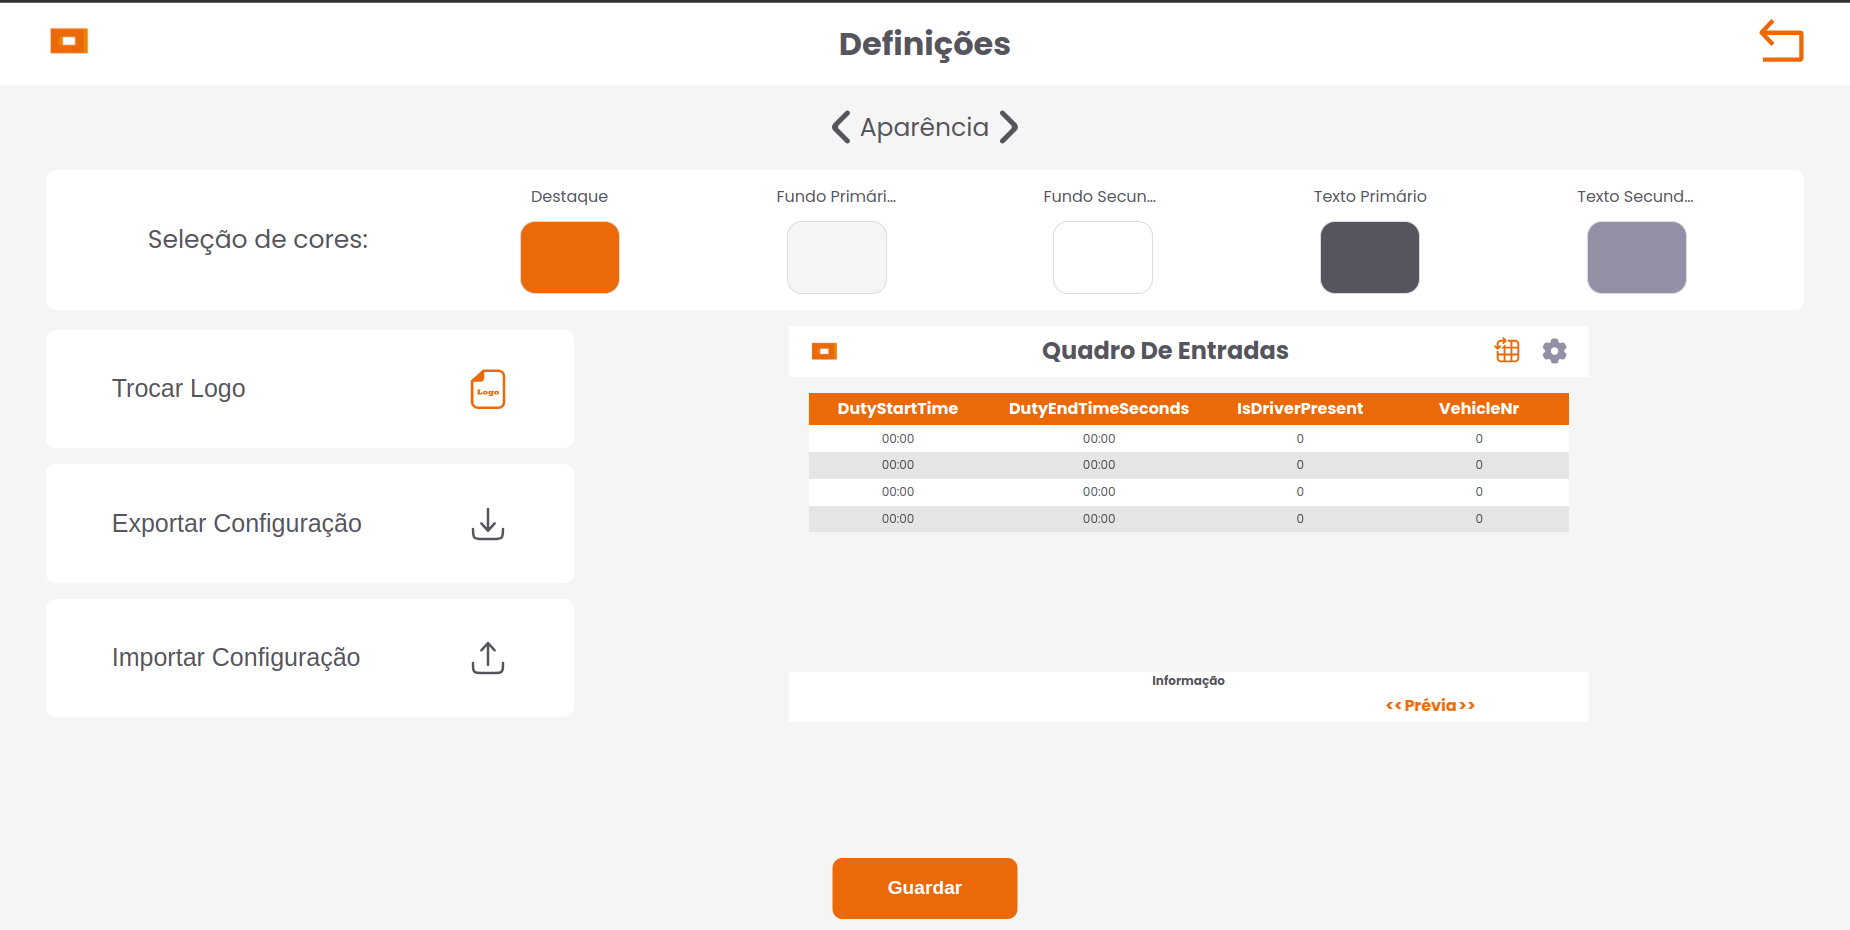
\includegraphics[width=1\textwidth]{aparencia}
            \caption{Settings page for customizing the appearance of the dispatch board system}
            \label{fig:settings_appearance}
        \end{figure}
        \vfill

        \begin{figure}[htbp]
            \centering
            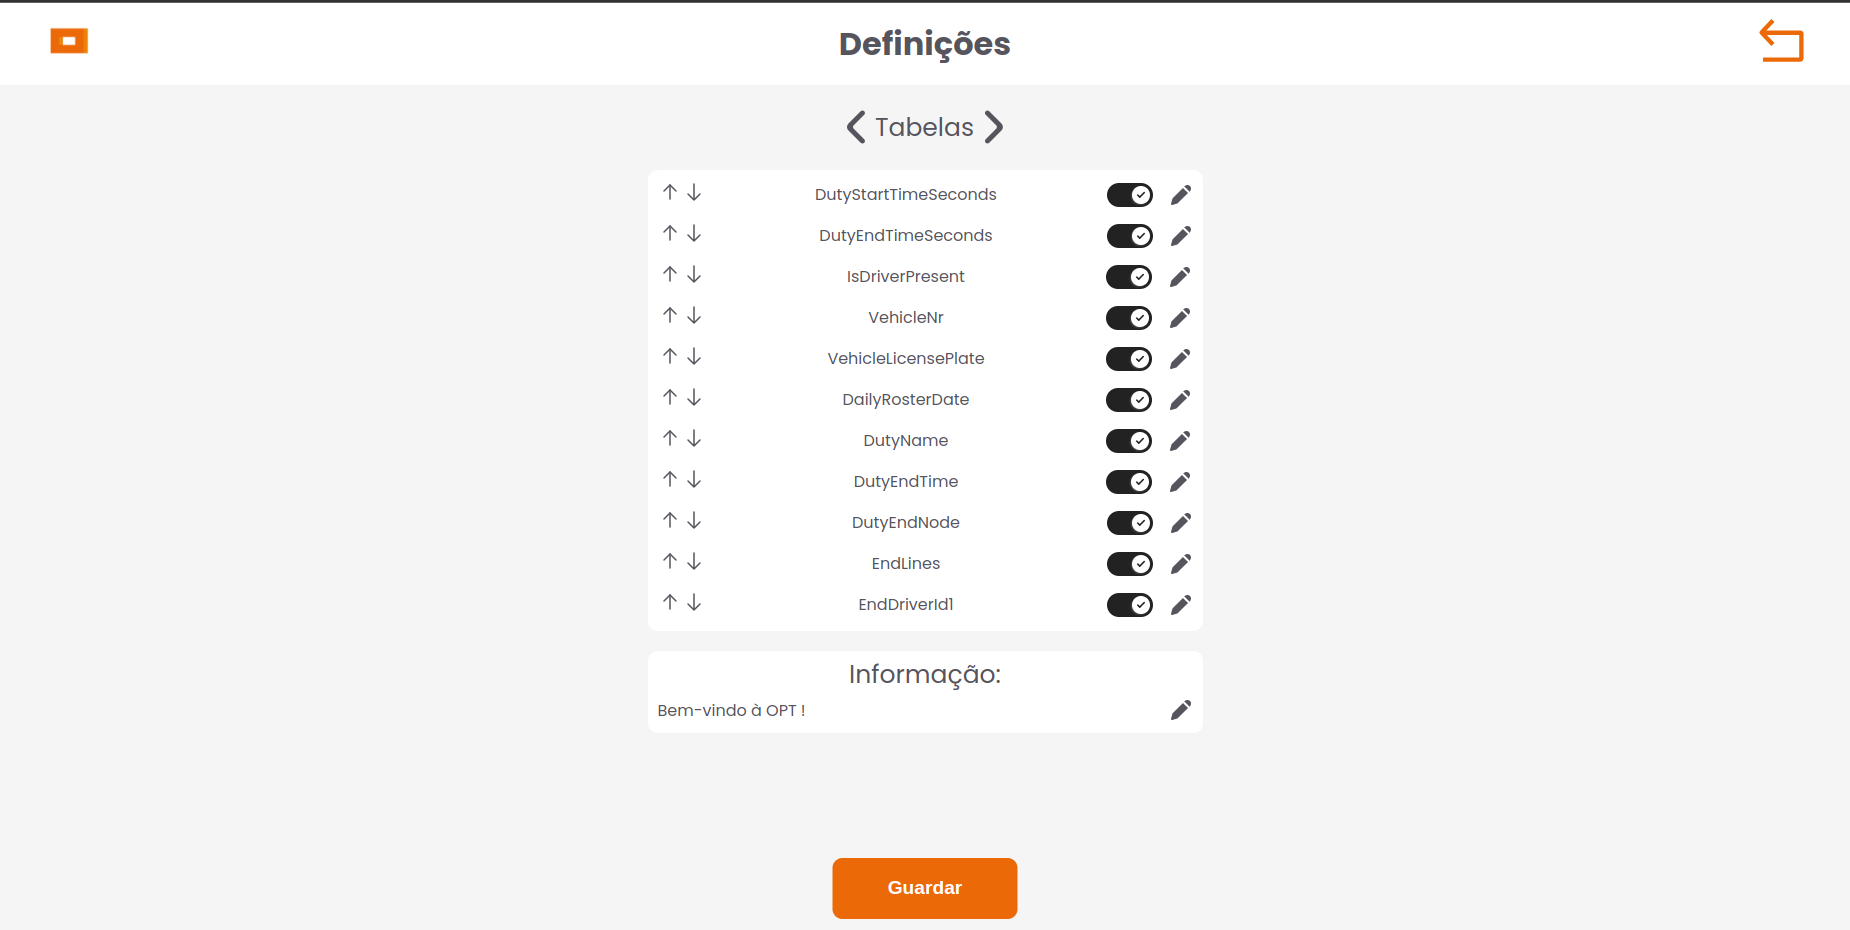
\includegraphics[width=1\textwidth]{tabelas}
            \caption{Settings page for customizing the tables in the dispatch board system}
            \label{fig:settings_tables}
        \end{figure}

        \subsection{Customization examples}

        Here, we present various customization examples to demonstrate the flexibility and adaptability of our application. Below, you will find screenshots of the Table of Entries and Table of Exits, each showcasing different customizations applied through the Settings Page. These examples illustrate how users can modify visual elements and functional components to align with their specific requirements and branding guidelines.
        \vfill
        \begin{figure}[H]
            \centering
            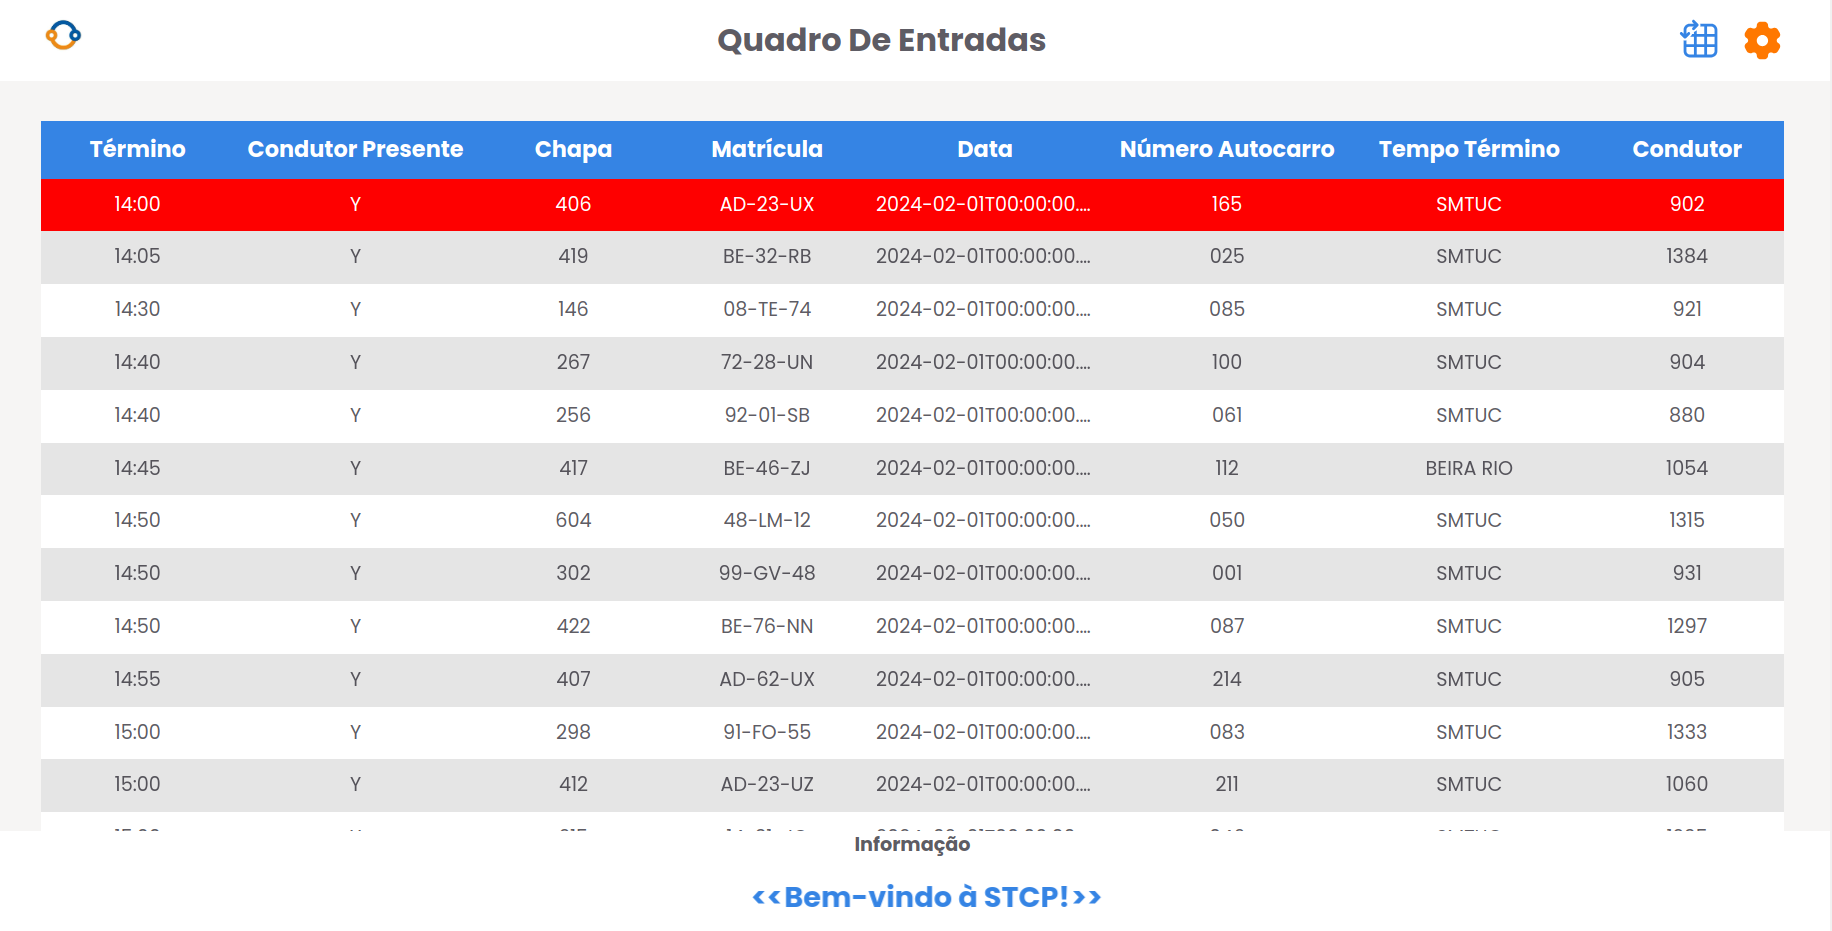
\includegraphics[width=0.95\textwidth]{table_of_entries_stcp1}
            \caption{Example of customization}
            \label{fig:table_of_exits_stcp1}
        \end{figure}

        \begin{figure}[H]
            \centering
            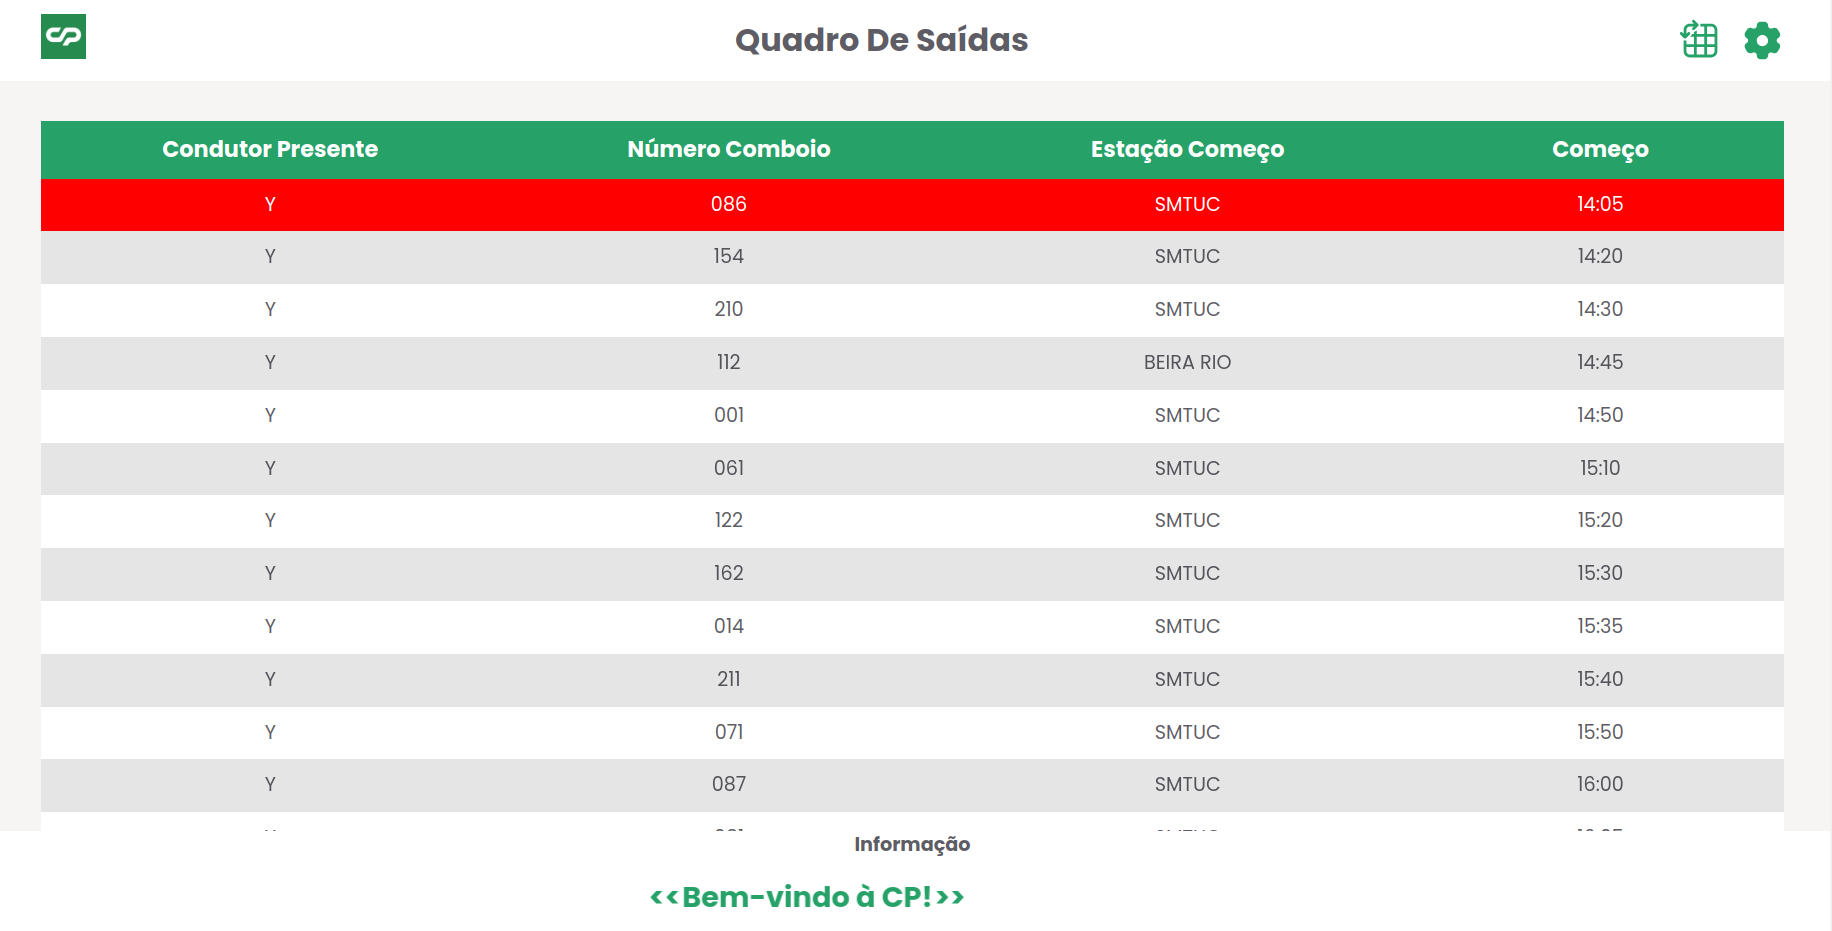
\includegraphics[width=0.95\textwidth]{table_of_exits_cp}
            \caption{Example of customization}
            \label{fig:table_of_exits_stcp1_}
        \end{figure}


        In these examples, I incorporated the STCP logo and color scheme to enhance the visual appeal.
        Additionally, I removed certain columns from the tables to create a cleaner layout, ensuring the information is more accessible and easier to read for users.

        \subsection{Validation}

        To ensure our project aligned with OPT's requirements, we sought guidance from our project manager, who provided weekly feedback for improvements. Our application was designed for larger screens, making testing on the TVs at OPT headquarters crucial. This allowed us to accurately gauge the dimensions of each compartment and validate our approach. 
        
        Since our application will be used by various companies, we tested possible configurations for different clients, such as STCP and CP, as illustrated. Additionally, we scheduled a test at STCP headquarters to obtain real-time feedback from users, further enhancing our application.


        \section{Conclusion}


        \subsection{Achieved Results}
        This project aimed to develop a modern dispatch board for public transport operators using web technologies. Our primary goal was to replace the outdated native software with a more user-friendly, web-based solution. 

        Key achievements include:

        \begin{itemize}
            \item \textbf{Web-Based Platform:} Migrated the dispatch board to a web-based language, enhancing expandability, debugging, and maintenance.
            \item \textbf{Customization:} Introduced extensive customization options for colors, layouts, and logos, with easy export/import functionality.
            \item \textbf{User Interface:} Developed a simple and intuitive interface using React with TypeScript and Next.js, ensuring ease of use.
            \item \textbf{Real-Time Updates:} Implemented real-time updates, ensuring transport operators have the most current information.
        \end{itemize}

        Challenges such as project setup and database communication were effectively addressed, leading to a streamlined development process. The final product, including tables for entries and exits and a comprehensive settings page, provides a robust, flexible tool for transport operators. The dispatch board dynamically displays schedules, highlights delays, and allows extensive customization, improving operational efficiency and user experience.


        \textbf{Group Contributions:}
        Every member of the group contributed well to the project's success, with each member taking on specific roles and responsibilities. The breakdown of contributions is as follows:
        \begin{itemize}
            \item António Ferreira: 25\%
            \item Cristiano Rocha: 25\%
            \item José Ferreira: 25\%
            \item Pedro Magalhães: 25\%
        \end{itemize}
         \subsection{Lessons Learned}

         Throughout this project, several important lessons were learned:

         \begin{itemize}
             \item \textbf{Effective Communication:} Regular meetings and open communication channels, such as Discord and GitHub, were crucial for progress and problem-solving and communicating with the OPT proponent.
             \item \textbf{Team Collaboration:} Working collaboratively, leveraging each member's strengths, and maintaining clear roles and responsibilities were key to the project's success.
             \item \textbf{User-Centered Design:} Prioritizing the end-users' needs, through intuitive interfaces and customization options, significantly enhanced the final product's usability and acceptance. This was especially important for transport operators who may not be tech-savvy.
             \item \textbf{Technical Proficiency:} Gained hands-on experience with modern web development tools and practices, particularly in React, TypeScript, and Next.js, which are relatively new technologies and were not covered in the academic curriculum.
         \end{itemize}


         \subsection{Possible Future Improvements and Further Work}

         While the project has successfully met its objectives, there are several areas for future improvement and further development:

         \begin{itemize}
             \item \textbf{Support for Smaller Devices:} Enhancing the application's responsiveness to support smaller devices like tablets and smartphones, ensuring a consistent user experience across all screen sizes. This was not a priority for this project, but it could be a valuable addition in the future.
             \item \textbf{Further Customization Options:} Expanding customization features to include additional settings and preferences for transport operators like font size, column width, finer color adjustments, etc.
             \item \textbf{User Feedback Integration:} Continuously gathering user feedback to inform iterative improvements and feature enhancements, through a feedback mechanism within the application.
             \item \textbf{Interoperability:} Enhancing interoperability with other systems and platforms used by transport operators to create a more cohesive ecosystem. For example, integrating a small app on the drivers' smartphones to receive notifications and updates and a way to communicate with the dispatch board if they are running late or on time.
         \end{itemize}

         In our opinion, the project was a very necessary improvement for the dispatch board system, as the old system was outdated and hard to maintain. The new system is much more user-friendly and customizable, providing a better experience for transport operators. In the development we deliberately chose to use Next.js and Prisma since they are modern and efficient technologies that we did not have the opportunity to work with during our academic curriculum. 
         
         In addition, we valued the experience to work in a real-world project, with a real client and real requirements, which was very enriching for our professional development. The way the OPT employees received us into their team was very welcoming and we felt like we were part of the team, which made the project even more enjoyable.

         In conclusion, the project successfully met its objectives, delivering a modern, customizable dispatch board system. The skills and knowledge gained during this project, including teamwork and technical proficiency, have been invaluable. The final product stands as a testament to our collective effort, providing a practical solution for public transport operators.        


        \bibliographystyle{plain}
        \bibliography{refs} % Entries are in the refs.bib file

        \end{document}